\documentclass{article}
\usepackage{amsmath}
\usepackage{amssymb}
\usepackage[legalpaper]{geometry}
\usepackage{graphicx}
\usepackage{bbm}
\usepackage[utf8]{inputenc}
\usepackage[T1, T2A]{fontenc}
\usepackage[english,russian]{babel}

\DeclareMathOperator{\diag}{diag}
\DeclareMathOperator{\Arg}{Arg}

\title{Примесь в простейшей модели топологического изолятора}
\author{Anikin Evgeny, 128}

\begin{document}
\maketitle
\section{Уровни энергии}
Гамильтониан простейшего топологического изолятора может быть записан в виде
\begin{equation}
    H = \left(\begin{matrix}
            \xi + \frac{1}{m}(2 - \cos{p_x} - \cos{p_y}) & 2t(\sin{p_x} - i\sin{p_y})   \\
            2t(\sin{p_x} + i\sin{p_y}) & - \xi - \frac{1}{m}(2 - \cos{p_x} - \cos{p_y}) \\
        \end{matrix}\right)
\end{equation}
Уровни энергии ---
\begin{equation}
    E_p^2 = (\xi + \frac{1}{m}(2 - \cos{p_x} - \cos{p_y}))^2 + 4t^2(\sin^2{p_x} + \sin^2{p_y})
\end{equation}
Если перейти из импульсного представления в координатное, то он превратится в гамильтониан
сильной связи. Гамильтониан примеси тогда можно записать в виде
\begin{equation}
    V = \Delta E (a_{00}^\dagger a_{00} + b_{00}^\dagger b_{00})
\end{equation}
Связанные состояния даются уравнением
\begin{equation}    
    \det{\left[\mathbbm{1} - \Delta E \int \frac{d^2 p}{(2\pi)^2} 
            \frac{\omega + \hat{H}}{\omega^2 - E_p^2}\right]} = 1
\end{equation}
В последнем интеграле (от матрицы) недиагональные члены из--за симметрии обращаются в ноль.
Таким образом, связанные состояния сводятся к уравнениям
\begin{equation}
    \label{integrals}
    \left[
    \begin{split}
        &\int \frac{d^2 p}{(2\pi)^2} 
            \frac{\omega + \xi + \frac{1}{m}(2 - \cos{p_x} - \cos{p_y})}
                 {\omega^2 - E_p^2} = \frac{1}{\Delta E},\\
        &\int \frac{d^2 p}{(2\pi)^2} 
            \frac{-\omega + \xi + \frac{1}{m}(2 - \cos{p_x} - \cos{p_y})}
                 {\omega^2 - E_p^2} = -\frac{1}{\Delta E},
    \end{split}
    \right.
\end{equation}
Эти интегралы можно взять приближённо в круге небольшого радиуса $p_{\mathrm{max}}$,
если учесть, что при малых $p$ спектр близок к 
коническому. После интегрирования получается
\begin{equation}
    G(\omega,0,0)_{11} = -\frac{1}{8\pi}\frac{1}{m(4t^2 + \frac{\xi}{m})}
        \left[ p_{\mathrm{max}}^2 + 
            \left(2m(\omega+\xi) - \frac{\xi^2 - \omega^2}{4t^2 + \frac{\xi}{m}}\right) 
                \log{\left(1 + \frac{\left(4t^2 + \frac{\xi}{m}\right)p_{\mathrm{max}}^2}
                                    {\xi^2 - \omega^2}\right)}\right]
\end{equation}
Конечно, интегралы из \eqref{integrals} можно взять численно. Для 
$\xi, m, t = -0.03, 0.1, 0.5$ компоненты функции Грина изображены на графике.

\begin{figure}[h]
    \centering
    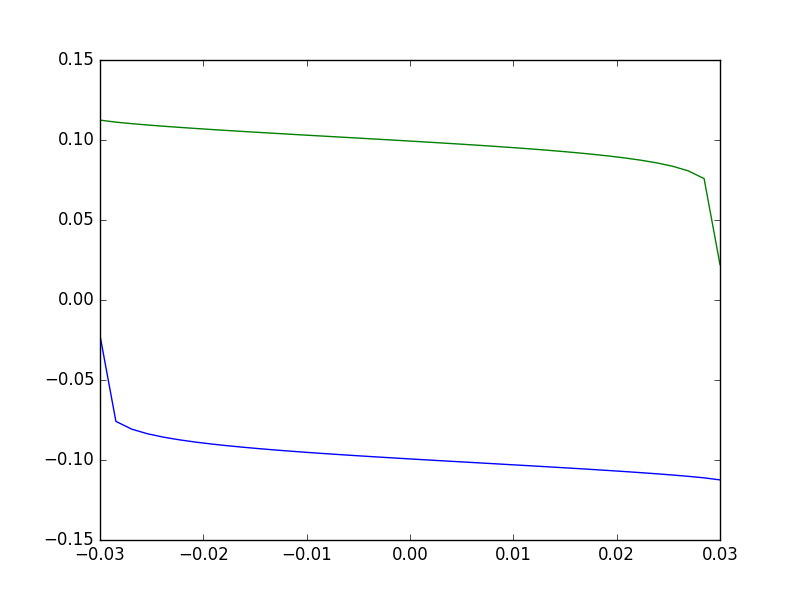
\includegraphics[width=0.8\linewidth]{green_functions.png}
    \caption{Компоненты функций Грина}
\end{figure}

Вычисление выше показывает, что происходит на краях этого графика. А именно, ``хвосты'' 
функций Грина растут логарифмически до бесконечности.
Таким образом, для малых $\Delta E < 0$ появляется одно связанное состояние около 
зоны проводимости. При дальнейшем росте возмущения появляется состояние около валентной зоны.

\section{Волновые функции}
Попробуем вычислить их в том же приближении. Волновые функции даются компонентами свободной
функции Грина:
\begin{equation}
    \Psi_{\alpha, i}(x) = G_0(x)_{\alpha i}
\end{equation}
Здесь $\alpha$ --- ``спинорный'' индекс, а $i$ --- индекс, соответствующий номеру волновой 
функции.

Функция Грина --- 
\begin{equation}
    G_0(x) = \int \frac{d^2 p}{(2\pi)^2} 
            \frac{\omega + \hat{H}}{\omega^2 - E_p^2} e^{ipx}
\end{equation}
Их можно вычислить с помощью формального трюка. Определим новую функцию
$F(x,y)$:
\begin{equation}
    F(x,y) = \equiv \int \frac{d^2 p}{(2\pi)^2} 
            \frac{e^{ip_x x + ip_y y}}{\omega^2 - E_p^2} 
\end{equation}
Несложно понять, что компоненты функций Грина выражаются (точными соотношениями)
 через $F(x,y)$. А именно,
\begin{equation}
    \label{differences}
    \begin{split}
        G_{11} & = (\omega + \xi) F(x,y) - 
            \frac{1}{m}(F(x+1,y) + F(x-1,y) + F(x,y+1) + F(x, y-1) - 4F(x,y))\\
        G_{21} & = -it(F(x+1,y) - F(x-1,y)) + t(F(x,y+1) - F(x,y-1))
    \end{split}
\end{equation}
С другой стороны, $F(x,y)$ может быть вычислена приближённо. Если разложить 
выражение в знаменателе около $p = 0$ и распространить интегрирование до $\infty$, то получится
сходящийся и берущийся интеграл.
\begin{equation}
    F(x,y) \approx -\int \frac{p\,dp\,d\cos{\theta}}{(2\pi)^2} 
        \frac{e^{ipr\cos{\theta}}}{\xi^2 - \omega^2 - (4t^2 + \frac{\xi}{m})p^2} = 
        -\frac{1}{2\pi} \frac{1}{4t^2 + \frac{\xi}{m}}
        K_0 \left(\sqrt{\frac{\xi^2 - \omega^2}{4t^2 + \frac{\xi}{m}}}R \right)
\end{equation}
Разности \eqref{differences} можно аппроксимировать производными. Пользуясь тем, что
$K_0(x)$ --- решение уравнения Бесселя, получим 
\begin{equation}
    \begin{split}
        G_{11} & = -\frac{1}{2\pi} \frac{1}{4t^2 + \frac{\xi}{m}}
        \left( \omega + \xi - \frac{1}{m} \frac{\xi^2 - \omega^2}{4t^2 + \frac{\xi}{m}} \right)
        K_0 \left(\sqrt{\frac{\xi^2 - \omega^2}{4t^2 + \frac{\xi}{m}}}R \right)\\
        G_{21} & = \frac{it}{\pi} \sqrt{\frac{\xi^2 - \omega^2}
                                     {(4t^2 + \frac{\xi}{m})^{3}}}
        K_0' \left(\sqrt{\frac{\xi^2 - \omega^2}{4t^2 + \frac{\xi}{m}}}R \right)e^{i\theta}
    \end{split}
\end{equation}
Найдём момент импульса найденных состояний. Оператор полного момента имеет вид
\begin{equation}
    J_z = x p_y - y p_x + \frac{1}{2}\sigma_z
\end{equation}
Несложно понять, что у двух найденных состояний полный момент равен $\pm \frac{1}{2}$.

Интересно также найти магнитный момент. Оператор магнитного момента ---
\begin{equation}
    m_z = \frac{e}{2c}(x v_y - y v_x) + \frac{e}{2m_0c} \sigma_z
\end{equation}
Операторы скорости в низшем порядке по импульсам ---
\begin{equation}
    \begin{split}
        v_x & = \begin{pmatrix} 
                -\frac{i}{m} \partial_ x & 2t \\
                2t & \frac{i}{m}\partial_x
              \end{pmatrix} \\
        v_y & = \begin{pmatrix} 
                -\frac{i}{m} \partial_y & -2it \\
                2it & \frac{i}{m}\partial_y
              \end{pmatrix} \\
    \end{split}
\end{equation}
Таким образом,
\begin{equation}
    m_z = \frac{e}{2mc}
            \begin{pmatrix}
               l_z & -2imt\cdot re^{-i\theta} \\
               2imt\cdot r e^{i\theta} & -l_z
            \end{pmatrix} + 
          \frac{e}{2m_0c} \sigma_z
\end{equation}

%Попробуем вычислить её в том же приближении (в кругу радиуса $p_{\mathrm{max}}$). 
%
%Начнём с $G_0(x)_{11}$. 
%\begin{multline}
%    G_0(x)_{11} = \int \frac{d^2 p}{(2\pi)^2} 
%        \frac{\omega + \xi + \frac{p^2}{2m}}{\omega^2 - \xi^2 - (4t^2+\frac{\xi}{m})p^2}
%            e^{ipr \cos{\theta}} = \\
%    = -\frac{1}{(2\pi)^2} \frac{1}{2m (4t^2 + \frac{\xi}{m})}
%        \int_0^{p_{\mathrm{max}}} pdp\,d\theta\,
%        \left(1 + \frac{2m(\omega+\xi) - \frac{\xi^2 - \omega^2}{4t^2+\frac{\xi}{m}}}
%                       {p^2 + \frac{\xi^2 - \omega^2}{4t^2 + \frac{\xi}{m}}}\right) 
%                        e^{ipr \cos{\theta}} = \\
%    = -\frac{1}{2\pi} \frac{1}{2m (4t^2 + \frac{\xi}{m})} 
%        \int_0^{p_{\mathrm{max}}} p\,dp\,J_0(pr)
%        \left(1 + \frac{2m(\omega+\xi) - \frac{\xi^2 - \omega^2}{4t^2+\frac{\xi}{m}}}
%                       {p^2 + \frac{\xi^2 - \omega^2}{4t^2 + \frac{\xi}{m}}}\right) 
%\end{multline}
%Последний интеграл состоит из двух слагаемых. Первое быстро осциллирует, и хочется верить,
%что это связано с обрезанием. Поэтому мы его выбросим. Второе можно вычислить, устремив 
%$p_{\mathrm{max}}$ к бесконечности. Такой интеграл есть в Градштейне--Рыжике, и в 
%результате получается
%\begin{equation}
%   G_0(x)_{11} = -\frac{1}{2\pi} 
%            \frac{2m(\omega+\xi) - \frac{\xi^2 - \omega^2}{4t^2+\frac{\xi}{m}}}
%            {2m (4t^2 + \frac{\xi}{m})} 
%            K_0 \left(\sqrt{\frac{\xi^2 - \omega^2}{4t^2 + \frac{\xi}{m}}}R \right)
%\end{equation}
%Теперь нужно вычислить $G_0(x)_{21}$.
%\begin{multline}
%    G_0(x)_{21} = \frac{1}{(2\pi)^2}
%                \int p\,dp\,d\theta\, \frac{2tpe^{i\theta} e^{ipr\cos{\theta}}}
%                            {\omega^2 - \xi^2 - (4t^2+\frac{\xi}{m})p^2} = \\
%                = \frac{-t}{2\pi^2(4t^2 + \frac{\xi}{m})}\int dp\,d\theta 
%                    \left(1 - \frac{1}{1 + \frac{4t^2+\frac{\xi}{m}}{\xi^2 - \omega^2}p^2}
%                    \right)
%                    e^{ipr\cos{\theta} + i\theta} = \\
%                =  \frac{-it}{\pi(4t^2 + \frac{\xi}{m})}\int dp\,
%                    \left(1 - \frac{1}{1 + \frac{4t^2+\frac{\xi}{m}}{\xi^2 - \omega^2}p^2}
%                    \right) J_1(pr)
%\end{multline}
%Здесь тоже возникает непонятное слагаемое, в основном пропорциональное $r^{-1}$. Его
%мы выбросим. Останется
%\begin{equation}
%   G_0(x)_{21} = \frac{-it}{\pi(4t^2 + \frac{\xi}{m})}
%                \sqrt{\frac{\xi^2 - \omega^2}{4t^2+\frac{\xi}{m}}}
%                   \int_0^{\infty} e^{-x - r\sqrt{\frac{\xi^2 - \omega^2}{4t^2+\frac{\xi}{m}}}
%                            \sinh{x}} \,dx
%\end{equation}
\end{document}
